\chapter{Vodík, jeho vlastnosti a typy}

Vodík (chemická značka \ce{H} z latinského \enquote{hydrogenium}\footnote{V roce $1783$ navrhl tento název francouzský chemik a biolog \textit{Antoine-Laurent de Lavoisier}, který odvodil z řeckého \enquote{ydor geinomai}, vodu tvořící.}) je nejrozšířenější prvek ve vesmíru a jedním z nejrozšířenějších na planetě Zemi. Tento velmi lehký a bezbarvý plyn nemá žádnou chuť ani zápach a je obtížně rozpustný v kapalných rozpouštědlech. Zároveň je kvůli své ne-toxicitě plynem bezemisním, a tedy při úniku z potrubí nenastává žádné znečištění životního prostředí. \cite{Greenwood1993}

Vodík je přítomen například ve formě vody (\ce{H2O}), zemního plynu (převážně \ce{CH4}), nebo metanolu (\ce{CH3OH}). Je nicméně schopný se vázat do sloučenin se všemi známými prvky periodické soustavy s výjimkou několika vzácných plynů. To je způsobené jeho nestabilní elektronovou konfigurací ($1\mathrm{s}^1 =$ jeden elektron ve valenčním orbitalu $1\mathrm{s}$), díky které také může existovat v až 40 různých formách, z nichž jsou mnohé detailně popsány. Za zmínku stojí především izotopy \textit{deuterium} \ce{^{2}_{1}H} a \textit{tritium} \ce{^{3}_{1}H}, které mají na rozdíl od lehkého vodíku \ce{^{1}_{1}H} v atomovém jádře kromě jednoho protonu ještě jeden, či dva neutrony. Na Zemi se však vodík v elementární formě ve velkém rozsahu nenachází, lze jej nalézt pouze vzácně, převážně v blízkosti vulkánů a sopek. V dalších kapitolách bude odkazováno především na plynnou formu dvouatomové molekuly \ce{H2}, neboli divodík, který se na Zemi nachází pouze v horních vrstvách atmosféry. \cite{Greenwood1993}

Vodík je nosičem energie, který je schopný přenést, nebo akumulovat množství energie přibližně $30\ \mathrm{kWh\krat kg^{-1}}$. \cite{Hytep} Pro další účely je nutné jeho výrobu uskutečnit přeměnou vhodné látky s použitím jiné formy energie, zejména elektrické a tepelné. \cite{Kadrnozka2006} Další vlastnosti vodíku jsou uvedeny v Tab. \ref{tab:vlastnosti_vodiku}.
\begin{table}[h]
    \centering
    \begin{tabular}{|c|c|}
        \hline
        \textbf{Vlastnosti} & \textbf{Hodnoty a jednotky} \\ \hline\hline
        relativní atomová hmotnost & $1,007825$ \\ \hline
        teplota tání & $13,957\ \mathrm{K}$; $-259,19\ \mathrm{^{\circ}C}$ \\ \hline
        výparné teplo & $0,117\ \mathrm{kJ\krat mol^{-1}}$ \\ \hline
        výhřevnost & $120\ \mathrm{MJ\krat kg^{-1}}$ \\ \hline
    \end{tabular}
    \caption[Vybrané atomové a fyzikální vlastnosti vodíku]{Vybrané atomové a fyzikální vlastnosti vodíku, převzato z \cite{Greenwood1993}.}
    \label{tab:vlastnosti_vodiku}
\end{table}

Dále je potřeba se seznámit se základními typy vodíku, na něž budeme odkazovat v následujících kapitolách. Dle barev rozdělené typy vodíku se používají k specifikaci jeho výroby a produkce oxidu uhličitého (\ce{CO2}) během výroby, vyjádřena jednotkami
\begin{equation*}
    \mathrm{gCO_{2,ekv.}}/\mathrm{MJ_{H_2}} \quad \mathrm{nebo} \quad \mathrm{gCO_{2,ekv.}}/\mathrm{gH_2},
\end{equation*}
tedy množství gramů ekvivalentu oxidu uhličitého vyprodukovaného při výrobě jednoho megajoulu energie obsaženého ve vodíku\footnote{Ekvivalent \ce{CO2} je míra vyjádření emisí skleníkových plynů pomocí daného množství oxidu uhličitého, které by mělo ekvivalentní příspěvek ke skleníkovému efektu jako dané množství jiných skleníkových plynů, např. metanu, nebo oxidu dusného. \cite{Trebicky2016}}, nebo množství gramů ekvivalentu oxidu uhličitého vyprodukovaného při výrobě jednoho gramu vodíku. Přepočet těchto jednotek je definován následující rovnicí \cite{Gericke2022}
\begin{equation}
    1\ \mathrm{gCO_{2,ekv.}}/\mathrm{MJ_{H_2}} = 0,\!12\ \mathrm{gCO_{2,ekv.}}/\mathrm{gH_2}
\end{equation}
Mezinárodní agentura pro energii \acs{IEA} a řada výrobců vodíku používají kromě barevného označování pro rozlišení typů technologií výroby a zpracování vodíku i alternativními názvy. Tyto názvy jsou převážně odvozené z angličtiny, jako třeba \textit{dekarbonizovaný}, nebo \textit{obnovitelný} vodík. Pro základní pochopení rozdílů a terminologie je v této kapitole definováno pouze pár základních typů.

\paragraph{Vodík vyráběný z fosilních paliv}
Vodík vyráběný z fosilních paliv bez zachycování oxidu uličitého je často nazýván \textbf{šedý} v případě výroby ze zemního plynu a ropných zbytků, nebo \textbf{hnědý} a \textbf{černý} v případě výroby z lignitu a černého uhlí. \cite{Griffiths2021} Právě na šedý vodík bude odkazováno v nadcházejících kapitolách nejčastěji, protože je při jeho výrobě vyprodukováno největší množství emisí ($90 \div 100\ \mathrm{gCO_{2,ekv.}}/\mathrm{MJ_{H_2}}$ \cite{Barth2016}) a zároveň jeho výroba tvoří necelých $63\%$ z celkové výroby vodíku ($\approx 60\ \mathrm{Mt_{H_2}}$ za rok), viz. Obr, \ref{fig:produkceH2}. \cite{IEAreview}
\begin{figure}[ht]
    \centering
    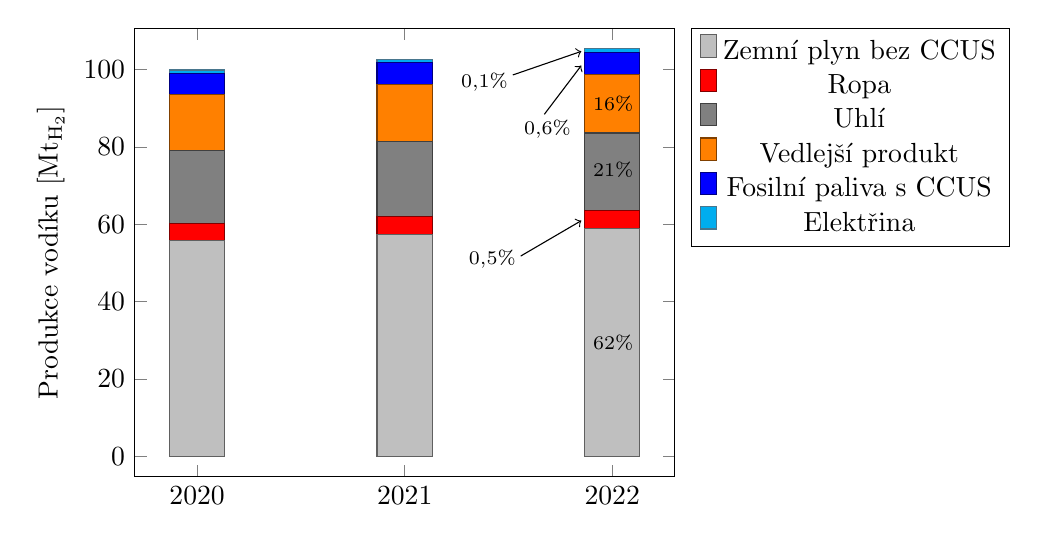
\begin{tikzpicture}
    \begin{axis}[
        ybar stacked,
	bar width=20pt,
        enlarge x limits=0.15,
        enlarge y limits=0.05,
        ymin = 0,
        legend entries={Zemní plyn bez CCUS,Ropa,Uhlí,Vedlejší produkt,Fosilní paliva s CCUS,Elektřina},
        legend pos=outer north east,
        ylabel={Produkce vodíku $[\mathrm{Mt_{H_2}}]$},
        symbolic x coords={2020,2021,2022},
        xtick=data,
    ]
    \addplot+[ybar,lightgray!50!black,fill=lightgray,text=black] plot coordinates {(2020,55.8) (2021,57.35) (2022,58.9)};
    \addplot+[ybar,red!50!black,fill=red,text=black] plot coordinates {(2020,4.5) (2021,4.625) (2022,4.75)};
    \addplot+[ybar,gray!50!black,fill=gray,text=black] plot coordinates {(2020,18.9) (2021,19.425) (2022,19.95)};
    \addplot+[ybar,orange!50!black,fill=orange,text=black] plot coordinates {(2020,14.4) (2021,14.8) (2022,15.2)};
    \addplot+[ybar,blue!50!black,fill=blue,text=black] plot coordinates {(2020,5.4) (2021,5.55) (2022,5.7)};
    \addplot+[ybar,cyan!50!black,fill=cyan,text=black] plot coordinates {(2020,0.9) (2021,0.925) (2022,0.95)};
    \end{axis}
    \node[font=\scriptsize] at (6.075,1.7) {$62\%$};
    \draw[->] (4.9,2.8) -- (5.67,3.25) node[below,xshift=-1.13cm,yshift=-0.25cm] {\scriptsize $0,\!5\%$};
    \node[font=\scriptsize] at (6.075,3.9) {$21\%$};
    \node[font=\scriptsize] at (6.075,4.73) {$16\%$};
    \draw[->] (5.2,4.6) -- (5.67,5.22) node[below,xshift=-0.43cm,yshift=-0.57cm] {\scriptsize $0,\!6\%$};
    \draw[->] (4.8,5.1) -- (5.67,5.4) node[below,xshift=-1.23cm,yshift=-0.15cm] {\scriptsize $0,\!1\%$};
\end{tikzpicture}
    \caption[Výroba vodíku podle technologií v období let 2020 až 2022]{Výroba vodíku podle technologií v období let 2020 až 2022 \cite{IEAreview}.} \label{fig:produkceH2}
\end{figure}

\paragraph{Nízkouhlíkový vodík}
Nízkouhlíkový, označovaný také \textbf{modrý} nebo dekarbonizovaný vodík je vyráběn stejnými metodami jako vodík šedý, ale vypouštění oxidu uhličitého do ovzduší je zpravidla eliminováno ukládáním pod zem pomocí \acs{CCS}, \acs{CCU} nebo \acs{CCUS} technologií, viz. Obr. \ref{fig:CCS}. Aby mohl být vyrobený vyrobený vodík takto nazýván, nesmí být překročena prahová hodnota vyprodukovaných emisí při jeho výrobě $36,4\ \mathrm{gCO_{2,ekv.}}/\mathrm{MJ_{H_2}}$\footnote{Prahovou hodnotu intenzity emisí pro nízkouhlíkový vodík definovala iniciativa \textit{CertifHy} v publikaci \cite{Barth2016} a je definována jako alespoň $60\%$ pokles emisí oproti emisím vyprodukovaných parním reformingem bez \acs{CCUS}.}. Od vyšších hodnot je vodík považován za šedý, nebo obecně za ne-nízkouhlíkový. \cite{Griffiths2021,VodikovaStrategie}
\begin{figure}[ht]
    \centering
    \begin{tikzpicture}
\node[inner sep=0pt] (obrazek) at (0,0)
    {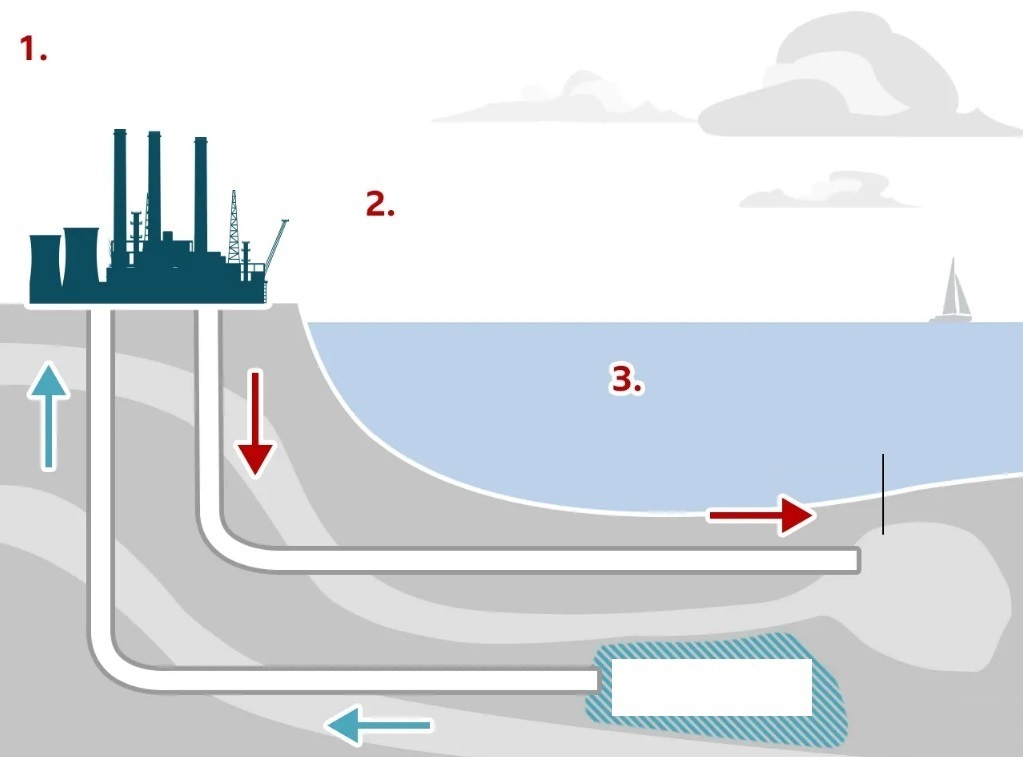
\includegraphics[width=0.8\textwidth]{figures/CCS.jpg}};
\node[font=\small\bfseries] at (2.2,-3.4) {Zemní plyn};
\node[font=\small\bfseries,align=center] at (-2.7,3.35) {Spalování zemního plynu\\na jednotkách výrobny};
\node[font=\small\bfseries,align=left] at (0.55,1.65) {Separování \ce{CO2}\\od ostatních plynů};
\node[font=\small\bfseries,align=left] at (3.4,-0.25) {Ukládání \ce{CO2} pod\\dno Severního moře};
\end{tikzpicture}
    \caption[Příklad technologie CCS zachycování a ukládání \ce{CO2} pod zem]{Příklad technologie \acs{CCS} zachycování a ukládání \ce{CO2} pod zem, převzato z \cite{CCS}.} \label{fig:CCS}
\end{figure}

\noindent
Zachycováním a ukládáním oxidu uhličitého lze v podstatné míře snížit uhlíkovou stopu vodíku (o $60 \div 95\%$ méně emisí oproti šedému vodíku) produkovaného tímto způsobem. \cite{Griffiths2021,VodikovaStrategie} Všechny výhody \acs{CCS} technologií jsou však zastíněny vysokou cenou těchto projektů. Nákladné je především separování oxidu uhličitého ze spalin. \cite{Seddon2022}

Vzhledem k tomu, že Česká republika je vnitrozemský stát nacházející se v mírném podnebném pásmu, má oproti přímořským státům\footnote{Mezi giganty ve využívání elektrické energie z obnovitelných zdrojů pro výrobu vodíku patří především Nizozemsko, jehož projekty budou představeny dále v této práci.} omezenou možnost využívat obnovitelné zdroje energie\footnote{V roce 2013 pocházelo pouze přibližně $13\%$ spotřebované elektrické energie v České republice z obnovitelných zdrojů. \cite{Tkac2017}} a technologie \acs{CCUS} v praxi. Produkce nízkouhlíkového vodíku je sice v souladu s klimatickými závazky České republiky, potažmo celé Evropy, ale jeho výroba je ze všech zmíněných konfigurací nejdražší, viz. Obr. \ref{fig:cenyH2}. \cite{VodikovaStrategie}

\paragraph{Obnovitelný vodík}
Obnovitelný, neboli \textbf{zelený} vodík je považován za \enquote{bezemisní} kvůli jeho výrobě pouze z obnovitelných zdrojů energie, převážně tedy elektrolýzou vody z elektřiny ze solárních a větrných elektráren, nebo např. reformováním biometanu, místo zemního plynu. \cite{Griffiths2021} Takto produkovaný vodík udává nadějnou perspektivu budoucnosti pro dekarbonizaci a tedy zbavení se závislosti na fosilních palivech v mnoha odvětvích průmyslu. Problém však představuje nákladnost jeho výroby, což má za důsledek vyšplhání ceny vodíku až na trojnásobek oproti konvenčnějším metodám výroby šedého vodíku v rafineriích, které si představíme v následujících kapitolách. \cite{Hytep} I kvůli faktoru jeho vysoké ceny je produkce zeleného vodíku stále minimální v porovnání s produkcí vodíku vyráběného z fosilních paliv. Obnovitelného vodíku se na světě vyrobí přibližně $4\%$ z celkové produkce, avšak valná většina z této části je vedlejším produktem z jiných technologií\footnote{Největší zástupce této skupiny je technologie výroby chloru elektrolýzou vodného roztoku chloridu sodného, kdy vznikají dva plyny — chlor (\ce{Cl2}) na kladné elektrodě a vodík na záporné elektrodě. Takto vyráběný vodík se dle barevného názvosloví označuje jako \textbf{bílý}. \cite{Hytep}}. \cite{Hytep} Cílená výroba vodíku za pomocí elektřiny pak tvoří pouze $0,1\%$ část, jak je znázorněno na Obr. \ref{fig:produkceH2}.

\paragraph{Ostatní typy a cenové srovnání}

Dle barev rozlišených typů vodíku je mnoho. Základní tři typy, na které je nejčastěji odkazováno jsou výše popsané \textbf{šedý}, \textbf{modrý} a \textbf{zelený}. Existuje pak řada dalších subtypů, za zmínku stojí například vodík \textbf{růžový}, který je vyráběn elektrolýzou vody z elektřiny pocházející výhradně z jaderných elektráren. Růžový vodík tedy lze zařadit do skupiny nízkouhlíkových vodíků, stejně jako například často opomíjený vodík \textbf{tyrkysový}. Tyrkysový vodík je vyráběn pyrolýzou metanu, která je výrazně méně energeticky náročná\footnote{Energetická náročnost pyrolýzy metanu činí $10 \div 30\ \unit{\kWh}/\unit{\kg}{\ce{H_2}}$, jenž je ve srovnání s elektrolýzou vody $50 \div 60\ \unit{\kWh}/\unit{\kg}{\ce{H_2}}$ v kontextu velkovýroby znatelně nižší. \cite{Diab2022}} než výroba zeleného vodíku elektrolýzou vody. Zároveň je při jeho výrobě oproti výrobě šedého vodíku vyprodukováno až o $90\%$ méně emisí, konkrétně pak cca. $7,6\ \mathrm{gCO_{2,ekv.}}/\mathrm{MJ_{H_2}}$. \cite{Diab2022}
\begin{figure}[h]
    \centering
    \definecolor{coalccs}{RGB}{178, 135, 240}
\definecolor{windoffshore}{RGB}{104, 244, 148}
\definecolor{windonshore}{RGB}{1, 173, 161}
\definecolor{solar}{RGB}{254, 211, 36}
\definecolor{jadro}{RGB}{227, 73, 71}

\begin{tikzpicture}
    \begin{axis}[
        ybar stacked,
        ymajorgrids,
        grid style={dashed,gray!30},
        width = 0.8\textwidth,
        height= 0.5\textwidth,
        bar width = 15pt,
        ymin = 0,
        ymax = 14,
        ylabel={Cena vodíku $[\mathrm{USD/kg_{H_2}}]$},
        legend entries={Zemní plyn bez CCUS,Zemní plyn s CCUS,Uhlí bez CCUS,Uhlí s CCUS,Elektřina z větrné elektrárny na moři,Elektřina z větrných elektráren na pevnině,Elektřina z fotovoltaiky,Elektřina z jaderných elektráren},
        legend style={at={(0.5,-0.1)},anchor=north},
        symbolic x coords={1,2,3,4,5,6,7,8},
        xtick=data,
        ytick={0,2,4,6,8,10,12,14},
        x tick label style={text=white}
        ]
    \addplot[transparent,fill=transparent,forget plot] coordinates {(1,1.2) (2,1.75) (3,1.9) (4,2.3) (5,3.55) (6,4.75) (7,3.7) (8,3.5)}; %odsazení sloupců
    
    \addplot[lightgray!50!black,fill=lightgray] coordinates {(1,4.6) (2,0) (3,0) (4,0) (5,0) (6,0) (7,0) (8,0)};
    \addplot[lightgray!50!black,pattern=north east lines,pattern color=gray,forget plot] coordinates {(1,0.5) (2,0) (3,0) (4,0) (5,0) (6,0) (7,0) (8,0)};
    
    \addplot[blue!50!black,fill=blue] coordinates {(1,0) (2,5.55) (3,0) (4,0) (5,0) (6,0) (7,0) (8,0)};
    \addplot[blue!50!black,pattern=north east lines,pattern color=blue,forget plot] coordinates {(1,0) (2,0.05) (3,0) (4,0) (5,0) (6,0) (7,0) (8,0)};

    \addplot[darkgray!50!black,fill=darkgray] coordinates {(1,0) (2,0) (3,2) (4,0) (5,0) (6,0) (7,0) (8,0)};
    \addplot[darkgray!50!black,pattern=north east lines,pattern color=darkgray,forget plot] coordinates {(1,0) (2,0) (3,1.1) (4,0) (5,0) (6,0) (7,0) (8,0)};

    \addplot[coalccs!50!black,fill=coalccs] coordinates {(1,0) (2,0) (3,0) (4,2.6) (5,0) (6,0) (7,0) (8,0)};
    \addplot[coalccs!50!black,pattern=north east lines,pattern color=coalccs,forget plot] coordinates {(1,0) (2,0) (3,0) (4,0.05) (5,0) (6,0) (7,0) (8,0)};

    \addplot[windoffshore!50!black,fill=windoffshore] coordinates {(1,0) (2,0) (3,0) (4,0) (5,8.5) (6,0) (7,0) (8,0)};

    \addplot[windonshore!50!black,fill=windonshore] coordinates {(1,0) (2,0) (3,0) (4,0) (5,0) (6,7.3) (7,0) (8,0)};

    \addplot[solar!50!black,fill=solar] coordinates {(1,0) (2,0) (3,0) (4,0) (5,0) (6,0) (7,7.6) (8,0)};

    \addplot[jadro!50!black,fill=jadro] coordinates {(1,0) (2,0) (3,0) (4,0) (5,0) (6,0) (7,0) (8,3.6)};

    \end{axis}
\end{tikzpicture}

    \caption[Porovnání nákladů na výrobu 1 kg \ce{H2} podle technologie výroby k roku 2022]{Porovnání nákladů na výrobu 1 kg \ce{H2} podle technologie výroby k roku 2022, převzato z \cite{IEAreview}.}
    \label{fig:cenyH2}
\end{figure}

Jak je patrné z Obr. \ref{fig:cenyH2}, produkce obnovitelného vodíku je až jednou tak nákladná oproti výrobě vodíku vyrobeného z fosilních paliv. To omezuje jeho dosavadní konkurenceschopnost, avšak predikce \acs{IEA} naznačují, že výrobní náklady obnovitelného vodíku využívajícího elektřinu z fotovoltaických elektráren by mohly v určitých regionech do roku 2030 klesnout až na $1,6\ \mathrm{USD/kg_{H_2}}$, tedy na aktuální cenu šedého vodíku. Zároveň by v lokalitách s dobrými větrnými podmínkami mohlo rovněž dojít k výraznému poklesu nákladů na výrobu obnovitelného vodíku. Ty by mohly v severozápadní Evropě dosáhnout hodnot kolem $2,1\ \mathrm{USD/kg_{H_2}}$. \cite{IEAreview}